\chapter{Workload Metrics} \label{ch:workload}
The paper presented in chapter 2 was written before the workload concepts and modeling language semantics had settled into their current form.  Jared et al. \cite{FVHMS}, in concert with this work, published a paper in the FVHMS proceedings that expands on the concepts in chapter 2 but is also slightly outdated.  Thus we feel it expedient to summarize those aspects of the language which are critical to our metrics before we present the metrics themselves.  To assist in this effort we have prepared a simple scenario which includes a partial model and illustrations of the DiRG, DiTG, and labeled state transition system.

\section{Example Scenario}
In this scenario there are two people, Alice and Bob.  Alice is standing next to Bob listening to a friend on her cell phone.  Bob suddenly remembers that he wants to ask Alice out.  Not noticing that Alice is listening to her phone Bob starts to ask Alice on a date.  When this happens Alice looks at Bob and points to her phone, signaling to him that she is on the phone.  Bob stops talking and decides between waiting for her to finish or walking away.  Eventually Bob walks away.

\subsection{Actors}
From the scenario above we chose to create three Actors: A) Alice, B) Bob, and C) Cell Phone.  Actors represent any aspect of the system that has state.  An Actor can be anything, in our example we have two humans and a cell phone.  We could also create a sub-Actor which is part of a larger Actor, such as Bob's hair, and give it states like messy or combed.  Actors can also be very abstract or very detailed.  The more states an Actor contains, the more expressive it becomes.

\begin{figure}[h]
\begin{center}
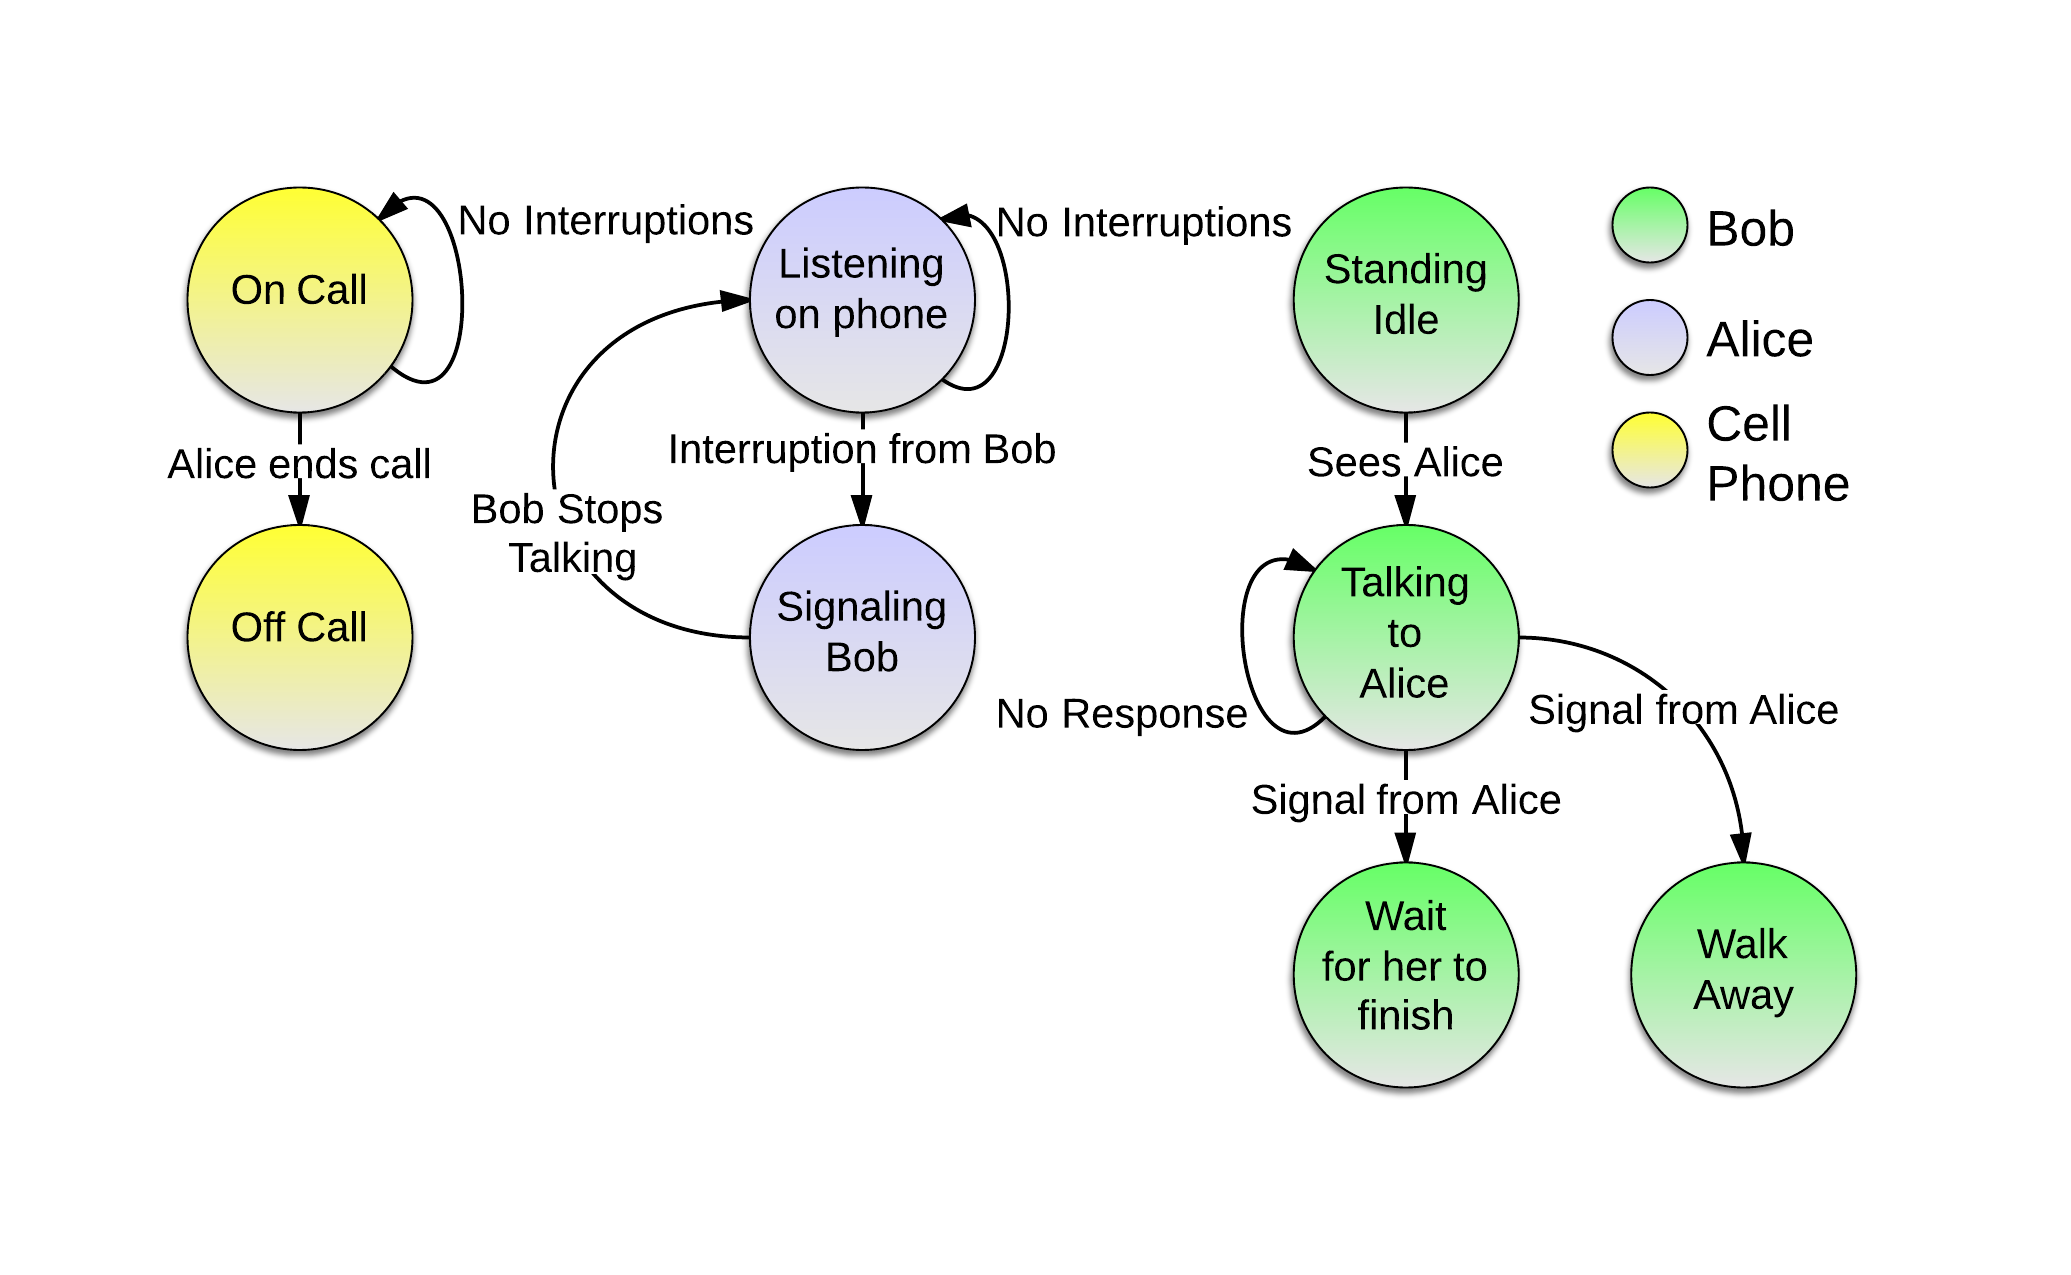
\includegraphics[width=\textwidth]{ab_dirg.png}
\caption{Directed Role Graph for Alice and Bob scenario}
\label{fig:ab_dirg}
\end{center}
\end{figure}

\subsection{DiRG}
We express an Actor as a Directed Role Graph (DiRG).  A DiRG represents how an Actor is allowed to flow between states.  Figure~\ref{fig:ab_dirg} shows the DiRGs for both Alice and Bob as a state transition system.  We see that Alice is initially in a {\em Listening on phone} state while Bob is in the {\em Standing idle} state.  Alice can either stay in the {\em Listening on phone} state, shown by the looping transition, or move into the {\em Signaling Bob} state.  Once in the {\em Signaling Bob} state her only choice is to stay there forever or to return to the {\em Listening on phone} state.  Individually these DiRGs are of little value, together they begin to express the larger system.  We see from the labels on the DiRG that Alice and Bob are interacting with one another and influencing the transitions of the other.  Before we discuss Actor transitions we must first define the inter-Actor relationship that allows Actors to influence one another.


\subsection{Channels}
We define these inter-Actor connections as Channels.  A channel is a uni-directional communication medium which allows an Actor to send information to another Actor.  Each Channel is composed of a source Actor, a target Actor, and a type.  The source Actor sends information as {\em output}, the target Actor receives the information as {\em input}, and the type specifies which communication medium is being used.  When describing the metrics we sometimes refer to the Channel source as the input source and the Channel target as the output target.  In the case of Alice and Bob we use audio, visual, and manual Channels\cite{wickens2002multiple}, the case study in chapter \ref{ch:UASinNAS} also uses a Data channel that represents network communication.  

We also designate that each Channel can represent multiple layers of communication.  To show this we will use the visual channel from Alice to Bob as an example.  We can express Alice's {\em output}, Bob's {\em input}, as two different layers on the visual channel, one for Alice's body language, and another for her facial expressions.  This allows us to explicitly set how much data is being sent over the channel, it also allows us to express multiple visual inputs for Bob without creating a {\em channel conflict}.  A {\em channel conflict} occurs when an Actor is receiving input from two or more channels of the same type.  In our example scenario Alice is listening to her cell phone which uses an audio channel.  At the same time Bob is talking to Alice on a different audio channel.  Because Alice is receiving {\em input} on multiple audio channels she has an audio channel conflict.  

\begin{figure}[h]
\begin{center}
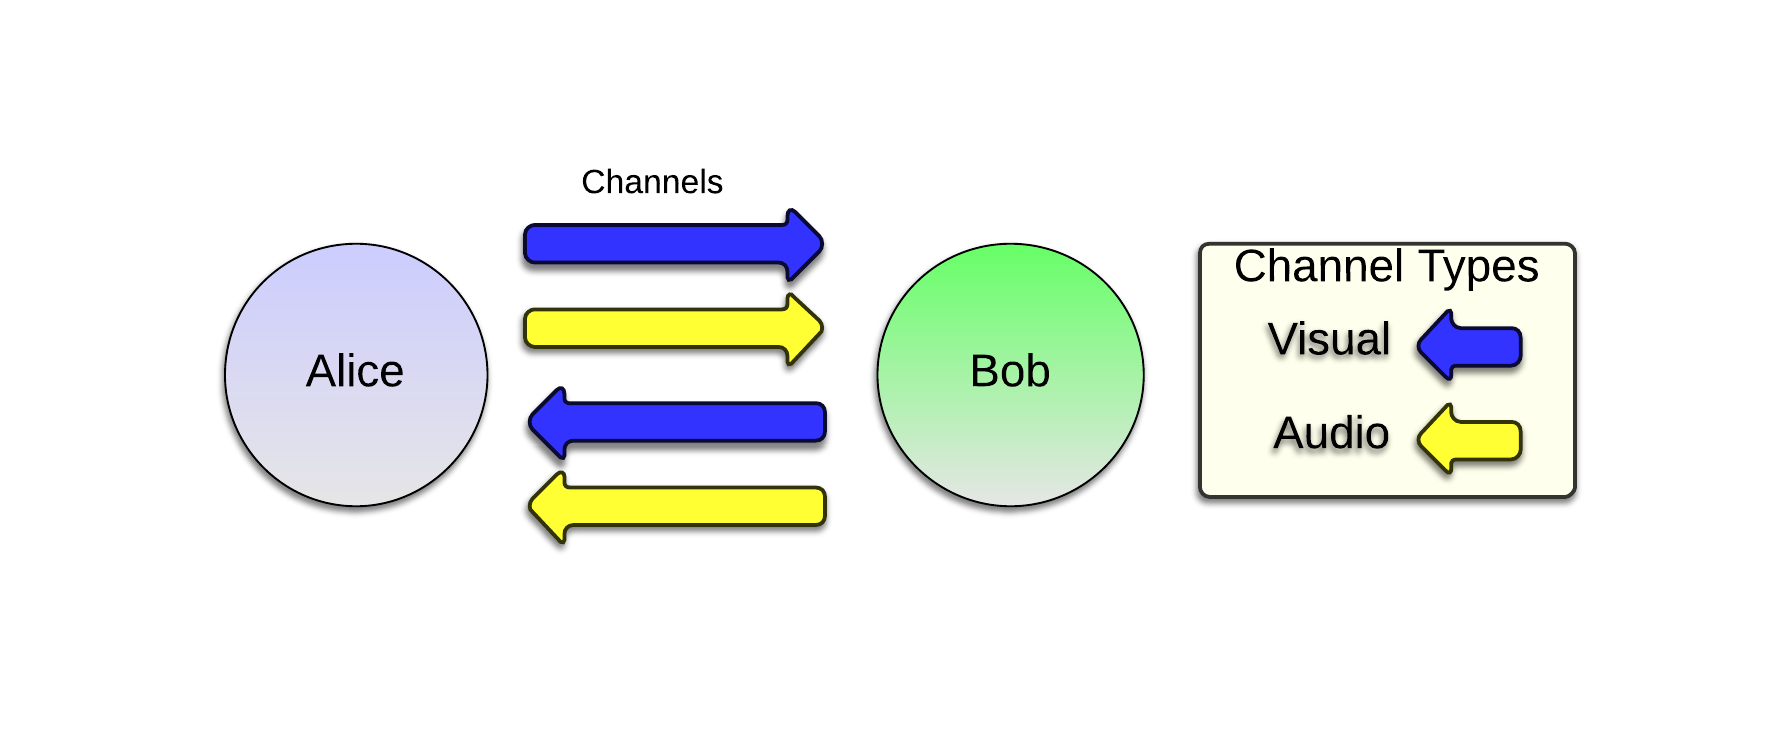
\includegraphics[width=\textwidth]{ab_ditg.png}
\caption{Directed Team Graph for Alice and Bob scenario}
\label{fig:ab_ditg}
\end{center}
\end{figure}

\subsection{DiTG}
To express a systems Channels we use a Directed Team Graph (DiTG)\cite{FVHMS}.  The DiTG defines all the channels that exist between the Actors within the system.  Figure \ref{fig:ab_ditg} shows the DiTG for our Alice and Bob scenario.  From the figure we can see that Alice has two channels to Bob, an audio and a visual and an audio channel to her cell phone.  We also see that Bob has two channels to Alice, an audio and a visual.  Lastly, the cell phone has an audio channel to Alice.  While the simplicity of this scenario makes it difficult to see the value of the DiTG, by combining the DiTG with the DiRG we have effectively constrained the Actor behavior and communication for the entire system.  With the constraints in place we are ready to define the behavior of the system, which we do with Transitions.


\subsection{Transitions}
Transitions represent an Actors behavior.  Transitions tells us about an Actors state, what caused the Actor to change state, and how that change effects the system.  Transitions are composed of a start state, an end state, a set of input equations, a set of outputs, a duration, and a priority.  The Transition start and end states are the states of the Actor and must not violate the DiRG.  

The Transition input equations are used to determine if the transition is enabled.  Each equation is composed of a source value, a predicate, and an expected value.  The source value is obtained from one of two sources, Channels or Memory.  Actor memory is an internal variable that allows an Actor to store and retrieve data.  For predicates we use equal to, less than, greater than, etc.  The structure of the input equations allows each equation to evaluate to a simple true or false.  If all input equations evaluate to true then the Transition is enabled.  

The Transition outputs contain all output generated by the transition as a set of target value pairs.  The target is the Channel or Memory variable that will receive the designated value.  The Transition duration is a range which represents the minimum and maximum number of time steps that a transition will remain {\em active} before it {\em fires}.  When an Actor decides to transition it selects an enabled transition to become {\em active}.  While a Transition is {\em active} the transition outputs are sent out but the Actor does not change state until the Transition {\em fires}.  We sometimes refer to inputs and outputs as being {\em active}, this implies that they are coming from an {\em active} Transition and that the value is not null.  The final Transition element is priority.  Priority reflects how important a Transition is to the Actor relative to the other Transitions.  If multiple Transitions are enabled the Actor will choose the Transition with the highest priority.

\begin{figure}[h]
\begin{center}
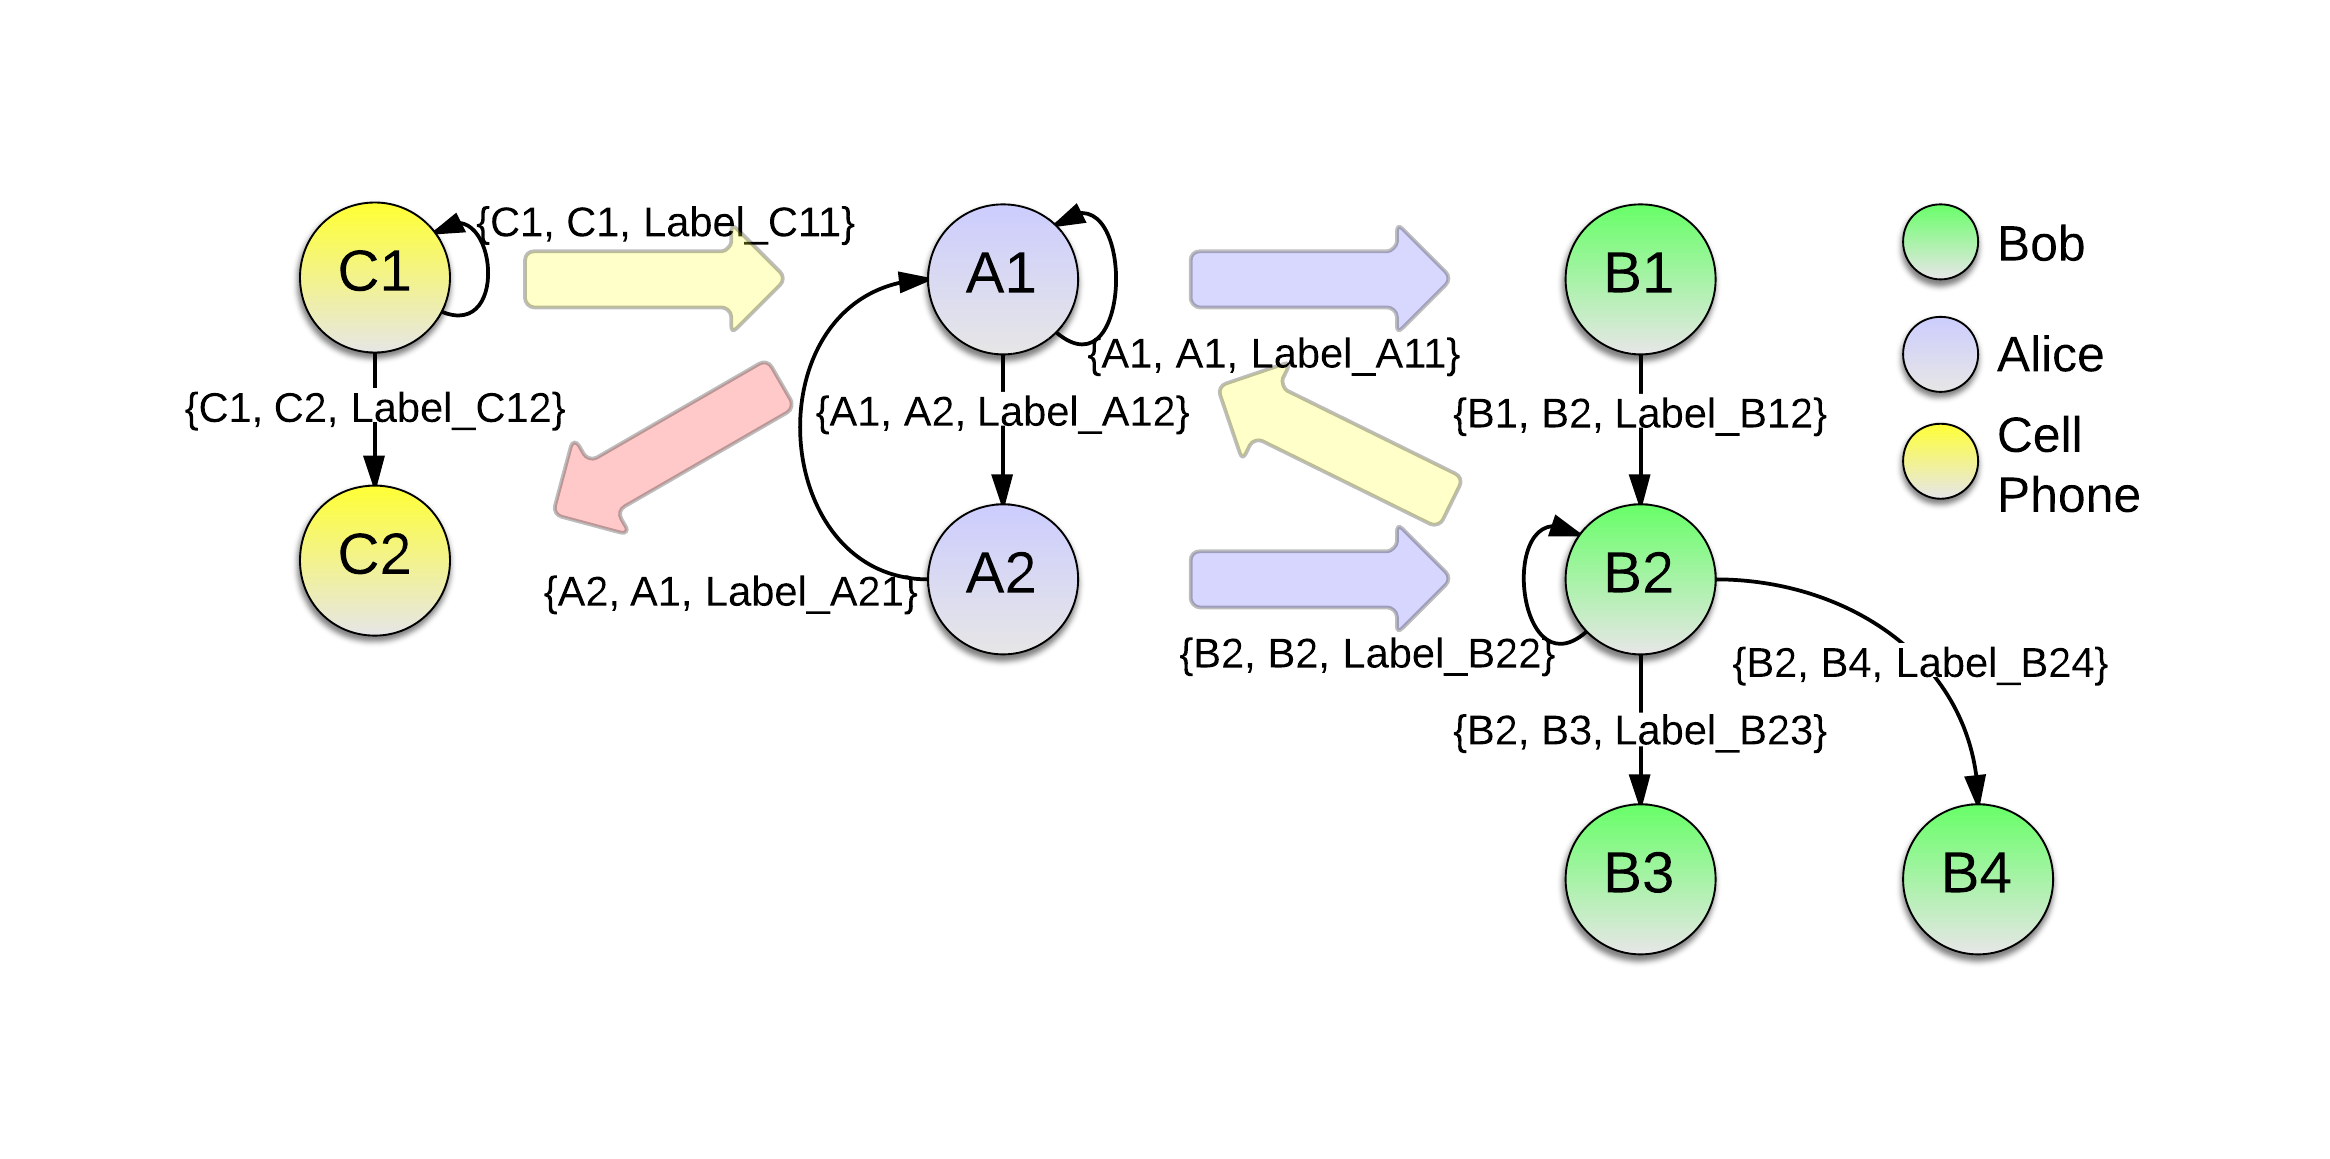
\includegraphics[width=\textwidth]{ab_lsts.png}
\caption{Labeled State Transition System for Alice and Bob scenario}
\label{fig:ab_lsts}
\end{center}
\end{figure}

\subsection{Labeled State Transition System}
The Model Abstraction Framework modeling language allows each of these concepts to be expressed in a model \ref{app:xmlparser}.  The model is then converted to a labeled state transition system that is sent to the simulator for metric collection.  We chose the labeled state transition system because the state transition system lends itself well to model checking while the label allows us to add specific data which relates to workload.  In our case the label translates directly to the transition input equations, outputs, duration, and priority.

In figure \ref{fig:ab_lsts} we can see that every transition has a label.  These labels are used by the simulator to determine if the transition is enabled, what channels will become {\em active}, and how long those channels should remain {\em active} before the state changes.  To make this clear we will describe $Label_A12$ of Alice's transition from the {\em Listening on phone} state to the {\em Signaling Bob} state.  From figure \ref{fig:ab_lsts} we see that when Bob is speaking to Alice there is an audio channel that is {\em active} (opaque yellow arrow).  The description on the transition implies that Bob's talking has somehow triggered the transition, to represent this in the label we create two input equations.  Audio channel from Bob does not equal null.  And audio channel from Cell Phone does not equal null.  This means that when Alice is listening to her cell phone if she hears Bob at the same time then this transition becomes enabled.  If she chooses to follow the transition then the transition becomes {\em active} and the transition outputs will become active.  In this case the output is a signal on the visual channel from Alice to Bob.  We will make the duration 5 seconds with a priority of 1.  

Now that we have a basic understanding of the data that the simulator has access to during the simulation we can now discuss how we translate this data into meaningful metrics.  We will first discuss our baseline workload metric.  Afterwards we will describe the two workload metrics we created as part of this work.


\section{Adapted Wickens' Metric}
Since we are interested in metrics that reveal human workload we have chosen to replicate Wickens' computational model~\cite{wickens2002multiple}, shown in equations~\ref{eq:wickens_model}-\ref{eq:resource_demand}, using data gathered from the Model Abstraction Framework.  Wickens' model is a measure of resource demand and overlap that has been shown to predict performance degradation, making it a good baseline metric for evaluating consistency with known high workload events and for comparison with the new metrics presented later in the chapter.  

Wickens' computational model is based on the concept of tasks, where a task is some arbitrary unit of activity.  Wickens' model calculates the resource interference between two tasks, a value that is closely related to mental workload~\cite{wickens2002multiple}.  The problem with using this computational model as a metric within the Model Abstraction Framework is the difference in the modeling paradigms.  In this work we abstract the notion of a task, relying instead on states and transitions to infer activity.  The challenge is to apply the task-based abstraction of Wickens' model to the state/transition based abstraction of the Model Abstraction Framework.

\begin{equation}
  W_{Orig}(T_{1}, T_{2}) = R_{Demand}(T^{1}, T^{2}) + R_{Conflict}(T^{1}, T^{2})
  \label{eq:wickens_model}
\end{equation}

\begin{equation}
  R_{Demand}(T^{1}, T^{2}) = T_{demand}^{1} + T_{demand}^{2}
  \label{eq:resource_demand}
\end{equation}

\begin{equation}
  R_{Conflict}(T^{1}, T^{2}) = \sum_{dimensions} \left\{
    \begin{array}{l l}
      1 & T_{x}^{1} = T_{x}^{2} \\
      0 & otherwise \\
    \end{array}
    \right.
  \label{eq:resource_conflict}
\end{equation}

Wickens' model ($W_{Orig}$), equation \ref{eq:wickens_model}, calculates the resource interference between two tasks, represented as $T^{1}$ and $T^{2}$, through the use of two components: resource demand ($R_{Demand}$) and resource conflict ($R_{Conflict}$).  Resource demand is a subjective measure of the cognitive resources required by a task.  In equation \ref{eq:resource_demand} we see that the resource demand of tasks $T^{1}$ and $T^{2}$ is calculated by summing the resource demand of both tasks.  To keep the model simple and intuitive Wickens limits $T_{demand}$ to a range of 0 to 2, where 0 is an automated task and 2 is a difficult task.  Thus $R_{Demand}$ will always be between 0 and 4.


\begin{figure}[h]
\begin{center}
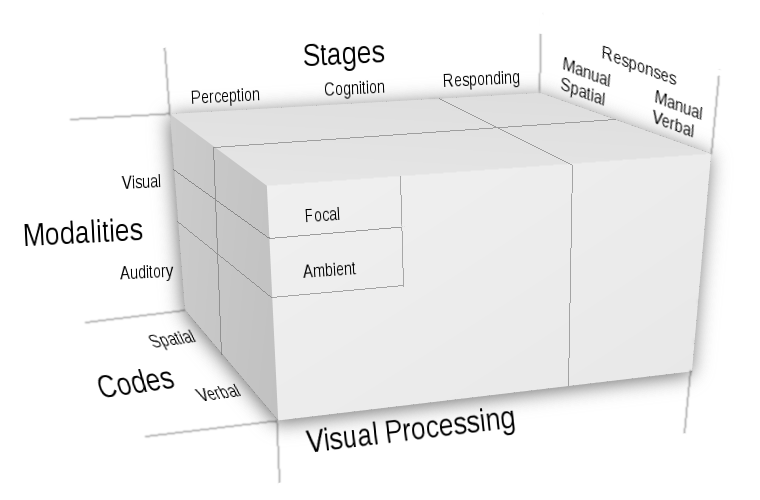
\includegraphics[width=6in]{multipleresourcetheory.png}
\caption{Multiple Resource Theory Dimensions~\cite{wickens2002multiple}}
\label{fig:multipleresourcetheory}
\end{center}
\end{figure}

For resource conflict two tasks are considered to have conflicting resources when they share resources within one of the dimensions illustrated in figure \ref{fig:multipleresourcetheory}.  In equation \ref{eq:resource_conflict} when $T_{x}$ represents the task resources for dimension $x$, then $R_{Conflict}$ is calculated by taking the sum of the total number of resource conflicts between two tasks.  Since there are only four dimensions $R_{Conflict}$ will always be between 0 and 4.  For example if $Task_{A}$ required a person to listen for distinct sounds while $Task_{B}$ required listening to a conversation, the resource conflict would be 2.  One in the {\em Stages} dimension for perception, and another in the {\em Modalities} dimension for auditory.  Since one deals with spacial sound and the other verbal sound no resources are shared in the {\em Codes} dimension.  As neither task dealt with visual perception there are no conflicts in the {\em Visual Processing} dimension.


  
\subsection{Actor Load}
To mimic resource demand within the Model Abstraction Framework we introduce the notion of Actor Load.  Actor Load represents an abstraction of the load an Actor is under while in a specific state.  Similar to resource demand in Wickens' model, Actor Load is a subjective value assigned by the modeler to each state in the system.  To make this value more intuitive and simple we have abstracted it into an integer value ranging from 0-4.  An Actor Load of 0 represents little to no load on the actor.  These are automated or transitional states where the Actor is idle or has minimal contact with the system.  An Actor Load of 4 represents simultaneously performing multiple high difficulty tasks.  These are states where an Actor is pushed to the limit of their cognitive capabilities. Any value between 0 and 4 is some combination of task difficulty and the number of tasks being performed.

\subsection{Determining Dimensional Conflicts}
To calculate the dimensionality of resource conflicts we need a way to determine when multiple tasks are being performed.  Since the Model Abstraction Framework does not define specific tasks we must find another method to approximate when multiple tasks are being performed.  We accomplish this by making the assumption that if an Actor has input from multiple sources then multiple tasks are being performed.

\begin{equation}
D_{Stages}(\Sigma, \Lambda) = \left\{ 
  \begin{array}{l l}
    1, \Sigma_{sources} > 1 & \quad \text{Multiple Input Sources}\\
    1, \Lambda_{targets} > 1 & \quad \text{Multiple Output Targets}\\
    0, otherwise
  \end{array}
  \right.
  \label{eq:stage_dimension}
\end{equation}

With this assumption we are ready to calculate dimensional conflicts as illustrated in Figure~\ref{fig:multipleresourcetheory}.  If $\Sigma$ represents the set of all inputs and $\Lambda$ the set of all outputs then we calculate the dimensional conflicts as follows.  For the Stages dimension (Perception, Cognition, Response), equation~\ref{eq:stage_dimension}, we check to see if there are multiple sources of {\em active} input or multiple output targets, not including memory inputs and outputs.  If multiple sources or targets exist then the stages dimensionality ()$D_{Stages}$) has a conflict.

\begin{equation}
D_{Modalities}(\Sigma, \Lambda) = \left\{ 
  \begin{array}{l l}
    1, \Sigma_{active}^{audio/visual} > 1 & \quad \text{Multiple Active Inputs}\\
    1, \Lambda_{active}^{audio/visual} > 1 & \quad \text{Multiple Active Outputs}\\
    0, otherwise
  \end{array}
  \right.
  \label{eq:modality_dimension}
\end{equation}

For the Modalities dimension (Audio, Visual), equation~\ref{eq:modality_dimension}, we check if there is more than a single {\em active} channel, input or output, for a specific channel type.  If there is then the modality dimensionality ($D_{Modality}$) has a conflict.

\begin{equation}
D_{Codes}(\Sigma, \Lambda) = \left\{ 
  \begin{array}{l l}
    1, \Sigma^{audio} + \Lambda^{audio} > 1\\
    1, \Sigma^{visual/manual} + \Lambda^{visual/manual} > 1\\
    0, otherwise
  \end{array}
  \right.
  \label{eq:codes_dimension}
\end{equation}

For the Codes dimension (Spatial, Verbal), equation~\ref{eq:codes_dimension}, we check that the total number of audio inputs and outputs is greater than 1 or that the total number of visual inputs, visual outputs, and manual outputs is greater than 1.  Since we do not specify different types of audio output we assume that all audio is verbal, likewise we assume that all visual/manual input and output is spacial.  If either check succeeds then the codes dimensionality ($D_{Codes}$) has a conflict.

\begin{equation}
D_{Visual Processing}(\Lambda) = \left\{ 
  \begin{array}{l l}
    1, \Lambda_{target}^{manual} > 1 & \quad \text{Multiple Manual Output Targets}\\
    0, otherwise
  \end{array}
  \right.
  \label{eq:focus_dimension}
\end{equation}

For the Visual Processing dimension, equation~\ref{eq:focus_dimension}, we check if there is more than one target for manual outputs.  We do not check inputs as we have no way of distinguishing if a visual channel is focal or ambient.  Instead we assume that manual outputs require visual focus, allowing us to determine if visual processing is split between multiple tasks.  If we have manual output to multiple targets then the visual processing dimensionality ($D_{Visual Processing}$) has a conflict

\subsection{Adapted Wickens' Model}
Using the Actor Load $A_{Load}$ and the adapted dimensionality conflicts we are now in a position to replicate $W_{Orig}$ within the Model Abstraction Framework.  As the model values are calculated differently than Wickens' model we will refer to this model as an adapted Wickens' model ($W_{Adapted}$).  The equation, shown in equation \ref{eq:adapted_wickens_model}, is as follows: given an actors State $S$ we can obtain the $A_{Load}$ as well as the inputs and outputs needed to calculate the four dimensionality values.  We obtain $W_{Adapted}$ by adding the $\A_{Load}$ of the state to the sum of the four dimensionality values.  This gives us a $W_{Adapted}$ between 0 and 8, just like $W_{Orig}$.

\begin{equation}
  W_{Adapted}(S) = S_{A_{ Load}} + D_{Stages}(S_{\Sigma}, S_{\Lambda}) + D_{Modalities}(S_{\Sigma}, S_{\Lambda}) + D_{Codes}(S_{\Sigma}, S_{\Lambda}) + D_{Visual Processing}(S_{\Sigma}, S_{\Lambda})
  \label{eq:adapted_wickens_model}
\end{equation}

Now that we have a baseline metric adapted from the related work to use as a baseline for consistency it is now time to describe two new workload metrics.

\section{Resource Workload Metric}

The resource workload metric attempts to measure the resource load an Actor is experiencing via inter-actor communications and memory access for each time step of the simulation.  The concept is based off of the cognitive workload category presented by Jared et al. \cite{FVHMS}.  For example, when Bob is talking to Alice she is processing input on multiple audio channels while also accessing any relevant memory.  Once Alice is alone again her resource workload will have decreased as she is only processing a single audio channel.

\begin{equation}
  Workload_{Resource}(State_{Current}, Inputs, Outputs) = State_{Actor Load} + ChannelConflicts(Inputs) + ResourceLoad(Inputs) + ResourceLoad(Outputs)
  \label{eq:resourceworkload}
\end{equation}

\begin{equation}
  ChannelConflicts(Inputs) = \sum_{ChannelTypes} \left\{
    \begin{array}{l l}
      1 & \sum Inputs^{ChannelType} \in Inputs > 1 \\
      0 & otherwise \\
    \end{array}
    \right.
  \label{eq:channel_conflict}
\end{equation}

\begin{equation}
  ResourceLoad(IO) = \sum IO_{Active} + \sum IO_{LayersRead} + IO_{MemoryRead} + \sum IO_{Active}^{ChannelTypes}
  \label{eq:resource_load}
\end{equation}

The resource workload metric, shown in equation \ref{eq:resourceworkload} is composed of three sub-metrics: channel conflicts, resource load, and Actor Load.  Channel conflicts occur whenever more than one active channel shares a type, such as an Actor receiving input on multiple audio channels.  Equation \ref{eq:channel_conflict} calculates the total channel conflicts by counting the number of $ChannelTypes$ that occur more than once in the set of all inputs.  Since we currently only allow visual and audio input for human Actors this value ranges from 0 to 2.  

Resource load attempts to quantify the load being placed on the Actor's resources.  We break the resource load into two parts, input and output, the final result being the sum of both parts.  Each part is calculated using equation \ref{eq:resource_load}, which adds the number of active channels, number of layers read, number of memory objects read, and the number of active channel types.  Actor Load is the same metric that is used in the adapted Wickens' metric and is included here because it is a direct reflection of the modelers belief of what the resource load is during this state.

To calculate the resource workload metric, inputs are gathered from each transition that is part of the current state.  The outputs are collected from the active transition.  We also use the Actor Load from the current state.  Channels are only counted once in the metric to prevent multiple transitions that share a Channel from skewing the metric.


\section{Decision Workload Metric}

The decision workload metric attempts to measure the complexity of the decision making process by measuring the size of the decision space for each time step of the simulation.  The concept is based off of the algorithmic workload category presented by Jared et al. \cite{FVHMS}.  For example, when Bob begins talking to Alice the added input enables an additional transition.  This means that Alice must now choose to keep trying to listen to the phone while Bob talks or signal Bob to stop talking, thus increasing her decision workload.  When Bob stops talking Alice's decision workload decrease as there is less input to process and fewer enabled transitions to choose from.

\begin{equation}
  Workload_{Decision}(State_{Current}, Inputs, Outputs) = EnabledTransitions_{State_{Current}} + Inputs_{Active} + Outputs + DurationComplexity(State_{Current})
  \label{eq:decisionworkload}
\end{equation}

To calculate the decision workload metric we use equation \ref{eq:decisionworkload} which is composed of four sub-metrics: decision complexity, input complexity, output complexity, and duration complexity.  The decision complexity represents how many options were available to choose from and is calculated as the number of enabled transitions for the current state.  In the case of Alice and Bob when Alice signals to Bob that she is on the phone Bob can choose to keep talking, stop talking and wait for Alice to finish, or walk away; thus Bob has a decision complexity of 3 while Alice is signaling.  

The input complexity represents the number of inputs that the Actor must process to make a decision.  It is calculated by summing the total number of inputs read by transitions, which includes active channels and memory variables.  Using the previous example, when Bobs decision complexity was three his input complexity could have been two, one from Alice's signal and another from a memory value representing how cute Alice is to Bob.  The output complexity is the same as the input complexity only the value is calculated from the outputs.

\begin{equation}
  DurationComplexity(State) = \log \frac{max(State_{Duration})}{60}
  \label{eq:duration_complexity}
\end{equation}

The duration complexity represents complexity that is related to the size of the task(s) being performed.  The underlying assumption being that difficult tasks take more time to complete than simple tasks.  While this assumption is not always true it is possible that some future variation of this metric may prove useful.  Due to the high variance and low trust associated with this metric we decided to normalize the duration complexity using equation \ref{eq:duration_complexity}.  By assuming that durations are in seconds and that any duration that is less than a minute has zero duration complexity we can convert durations into minutes and then use a logarithmic scale for the final value.  While the diminishing returns of this model allow us to show the duration complexity within the context of our other metrics it does not account for human fatigue and other factors associated with long running tasks.  We leave it up to future work to determine the usefulness of duration complexity and how it should be calculated.



